% Created 2016-11-09 Wed 18:12
\documentclass[11pt]{article}
\usepackage[utf8]{inputenc}
\usepackage[T1]{fontenc}
\usepackage{fixltx2e}
\usepackage{graphicx}
\usepackage{longtable}
\usepackage{float}
\usepackage{wrapfig}
\usepackage{rotating}
\usepackage[normalem]{ulem}
\usepackage{amsmath}
\usepackage{textcomp}
\usepackage{marvosym}
\usepackage{wasysym}
\usepackage{amssymb}
\usepackage{hyperref}
\tolerance=1000
\usepackage[margin=1in]{geometry}
\author{Jolly Roger Insecurity}
\date{}
\title{An Introduction to Reverse Engineering with IDA}
\hypersetup{
  pdfkeywords={},
  pdfsubject={},
  pdfcreator={Emacs 25.1.1 (Org mode 8.2.10)}}
\begin{document}

\maketitle
\tableofcontents

\section{Introduction}
\label{sec-1}
IDA and IDA Pro are disassemblers that will make your life much easier when
it comes to disassembling executables as well as understanding the underlying
code. IDA, short for \emph{Interactive DisAssembler}, allows a reverse engineer to
not only see disassembled code, but to modify it in such a way to make
understanding the disassembly much easier at a glance. IDA will attempt to
identify variables while allowing a reverse engineer to rename variables and
functions as well as propagating those changes throughout the disassembly. IDA
even allows the user to make comments on the disassembly.

IDA allows for disassembly of not only x86 binaries--it supports a number of
other architectures such as ARM, MIPS, and others. Many CTFs will provide
challenges for somewhat esoteric architectures, and we need a tool that can
handle those. If a particular architecture is unsupported by IDA, it provides
for a rich plugin interface that would allow us to write add-ons to handle
that architecture.

Finally, IDA has a well-integrated debugging system that allows for
debugging on the local host as well as providing an interface for remote
debugging such as that which can be done with \emph{gdbserver}.

\section{IDA in CTF}
\label{sec-2}
For our purposes, IDA is an invaluable tool for both reverse engineering and
exploitation exercises. We will use it for disassembly, local and remote
debugging, and CTF vulnerability research/exploit development.

\section{Opening IDA and loading a file}
\label{sec-3}
Go ahead and open IDA. If you're not sure whether you need to open the version
for 32 or 64 bit binaries and you have IDA Pro, open the 64-bit version.

Immediately you may see a box with information about the IDA license. Click OK
or ignore it, and you'll see a box with three options: new, go, and previous.
"New" will prompt you to open a binary to disassemble. "Go" will open IDA to a
blank interface. "Previous" will allow you to open a previous IDA database
listed in the menu below.

Go ahead and choose "New". You have been provided with a file titled
"gametime.exe". This is part of a challenge from the CSAW CTF 2016
qualification event. Navigate to and open this file.

At this point, you should run the executable for testing--if on Windows, you
should be able to run it natively. If you're on Linux or MacOS, you'll need to
run it either through a translation layer such as Wine or through a virtual
machine running Windows. You'll notice that it's a simple game that requires
prompted well-timed keypresses to play and win.

\begin{figure}[H]
\centering
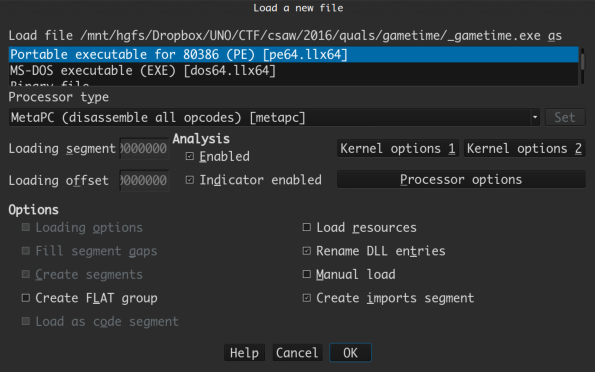
\includegraphics[width=.9\linewidth]{./gametime_load_prompt.png}
\caption{\label{Figure-1}IDA file loading screen}
\end{figure}

Back to IDA, you'll see a window that should look similar to Figure 1 above.
The list at the top of the window allows you to pick an IDA loader for the
file type that IDA has detected (such as a PE file, in this case), or you can
choose to simply load the file as data, in which case IDA will not parse it
to find code sections, data, etc--if you require, you would need to do this
yourself. However, if it's not already selected, choose the PE (Portable
executable for 80386) option.

Secondly, you'll be able to select the processor type. IDA should have
automatically selected MetaPC. This is fine in this case, however, depending
on your file type, and whether or not IDA has been able to automatically
determine the file type and processor, you may need to select a particular
processor type for your binary such as ARM, MIPS, Motorola 6803, etc. If
MetaPC has not been selected, choose that option.

Those are the two primary options--we need not select any others, but we'll
describe some others. Depending on how executables are normally loaded on
their system, you may need to adjust the loading segment and offset such that 
IDA displays and interprets the executable as being loaded into a particular
area of memory. If you were to disable program analysis, IDA would not 
disassemble the program code or populate subroutine listings, variables, or
other attributes. With "manual load", you are given more options in loading
such as where to base the file, which sections of the file to load, etc. You
can choose to specifically load resources such as images into the IDA database
(something you might wish not to do depending on size and relevance to the
disassembly).

Other options in the loading prompt you may need to understand for other
files, but for now, we'll move on. Go ahead and click "OK". IDA will proceed
to load the file.

\section{Taking an initial look at the disassembly}
\label{sec-4}
When it loads, you should see a sidebar that contains function names on the
left side. If you don't see it, typing "Shift+F3" should open a function
window. While the number of functions makes this executable look huge, you can
find the core logic of most compiled executables in the main function. In this
case, the function should be titled "\_main", and should be near the top of
the sidebar. If not, click on a function within that sidebar, and hit Alt+t to
search for "\_main". Once you find it, double-click on it, and main's code
should be visible within the main window.

If the main window shows a simple linear code listing rather than a graph,
click within the primary window and hit the spacebar. At this point, you
should see a graph view, which can be particularly helpful for visualizing a
program's control flow. Each function has its own code graph, and the blocks
within are divided by code jumps. For conditional jumps, the green (or other,
you may need to check settings) arrow should point to target blocks for which
the jump is taken, and the red arrow points to blocks for which the jump is
not taken (if viewing a simple code listing, the red arrow targets should
generally immediately follow the conditional jump).

You'll notice that at the top of the function, IDA has given you its guess as
to main's parameters. It has also enumerated a number of local variables and
arguments based upon patterns of stack allocation and local memory access. As
mentioned before, you can change the names of these variables and arguments as
you see fit, and the changes should propagate throughout the scope of these
variables and arguments within this function as well as possibly outside (for
function calls).

Scroll through the code for \_main, taking note of the various strings
referred to by various offsets pushed to the stack--these strings will be
partially visible in the graph through automatically populated comments, so
you don't need to follow the offsets to read the strings like you would in a
debugger like GDB.

At this point, you may want to run gametime.exe again. Take a note of the
strings that you see as you play through it, and see if you can see any of
those strings in the main function--they are there. Also, note that many of
these strings are pushed to the stack as arguments to one particular function.
Marked "sub\_401A73" in the example listing, let's proceed with the assumption
that the function at 0x401A73 is a custom print function due to the context of
its usage. Assumptions such as this can be dangerous to make (especially in
malware analysis), but remember that we're competing in a CTF, and must make
the best of our time.

While remaining in the main function, click on any line that calls sub\_401A73,
making sure that you click on the particular part of the line that says
"sub\_401A73". Now hit the "n" key. A box will pop up that asks for a new name
for the function, so let's call it "custom\_print". Type that into the box and
click "OK". You'll note that every reference to that function (within main and
elsewhere) now refers to it by "custom\_print" rather than "sub\_401A73". Now
you'll no longer need to remember the function by the old name, and scanning
through code that frequently references that function should be much easier.

\section{Searching the database}
\label{sec-5}
We could continue to disassemble the main and other functions to better nail
down functionality, but again, we're short on time. While playing
gametime.exe, you may have noticed a particular string pop up on failure:
"UDDER FAILURE!" with a link. Let's find where that string pops up in the
program. We need to navigate to the \emph{strings} subview. To find it, you can
either type "Shift+F12" or click on the View menu, mouse down to "Open
subviews", and then follow that to "Strings".

Once the strings window is up, click somewhere within it, and then type
"Alt+t". You should see two separate occurrences of that string. If you don't
see the second, typing "Ctrl+t" will continue a prior search, and you should
see the second occurrence. Double-click on one, and IDA will navigate to it in
the executable, in the .rdata section. Following the string, you'll see a note
that there's a cross reference, referencing it as data: "DATA XREF: sub\_\ldots{}".
Double-clicking on the name of the subroutine will take you to the reference
to the string in code.

\section{Patching the database}
\label{sec-6}
If you follow both occurrences of the string to their cross references, you'll
notice that both lie in a block of code following a conditional jump. They're
being pushed as arguments to the custom print function, so evidently the
preceding conditional jump has resolved for the failure condition. What if we
switch these?

While many reverse engineering challenges require the solver to RE code that
will dynamically build the flag based upon user input, that may not always be
the case. If that is the case here, our job is made more difficult. To save
time, let's proceed initially with the assumption that nothing is calculated
from our input, and that the program simply checks to see if we provided the
right input at the right time.

So if that's true, then all we need to do might be to simply force control
flow into the success block--we can do so by flipping the conditional or
changing it to an unconditional jump into the correct block.

If you're not looking at one of the pushes of an "UDDER FAILURE!" string,
navigate back to one now. Click on the line of the conditional jump that
precedes the "UDDER FAILURE" block of code. Now click on the Edit pulldown
menu at the top, and mouse over "Patch program". Within that submenu, click on
"Assemble\ldots{}". A window should pop up with a text box containing the jump
instruction. Changing the conditional jump mnemonic either to its opposite to
force success upon failure of hitting the right key in time or to "jmp" should
accomplish our goal. Hit "OK". If you have the assembly listing up you should
notice the change in the code, and if you have the graph view up, you'll see
that the graph has rearranged itself, and the failure block will likely now be
missing. If the "Assemble instruction" menu remained up after hitting "OK",
clicking "Cancel" should close the window while leaving the change intact.

Don't forget now to make the same change to the other occurrence of "UDDER
FAILURE!"!

Click on the Edit menu again, mouse through "Patch program", and click on
"Apply patches to input file\ldots{}". This will bring up a dialog box. Before
clicking "OK", you may want to make a copy of the executable, or check the
"Create backup" box to do the same in IDA. Once you've backed up the original
executable, clicking "OK" will write the changes to the executable.

\section{Capturing the Flag}
\label{sec-7}
Now run the executable again. Depending on how you patched it, pressing keys
may not matter (though if you reversed the conditional, you may just want to
keep your hands off the keyboard). Wait a while, and eventually the flag is
output--it's a non-standard flag format for this competition, but you'll know
the right one.
\section{Keyboard Shortcuts}
\label{sec-8}
Provided is a table of useful shortcuts. Many of these are not touched upon,
and some of them (particularly keys used for commenting the disassembly) are
vital functions.

\begin{center}
\begin{tabular}{ll}
\hline
Task & Command\\
\hline
Comment a line & \texttt{:}\\
Add repeatable comment (will propagate to anything referencing that line) & \texttt{;}\\
Search current subwindow & \texttt{Alt+t}\\
Continue search & \texttt{Ctrl+t}\\
View cross-references to item at cursor & \texttt{x}\\
Convert data at point to code & \texttt{c}\\
Undefine at point & \texttt{u}\\
Rename & \texttt{n}\\
Convert at point to data & \texttt{d}\\
Convert at point to ASCII string & \texttt{a}\\
Jump to address & \texttt{g}\\
\hline
\end{tabular}
\end{center}

For more function shortcuts, functions available in the IDA pulldown menus
with shortcuts will generally show the shortcut in the menu. For example,
there are a myriad of search types available in the Search pulldown menu, and
almost each has its own shortcut.
% Emacs 25.1.1 (Org mode 8.2.10)
\end{document}